\documentclass[11pt]{article}

% Standard packages for arXiv submission
\usepackage[utf8]{inputenc}
\usepackage[T1]{fontenc}
\usepackage{lmodern}
\usepackage{amsmath}
\usepackage{graphicx}
\usepackage{dcolumn}
\usepackage{bm}
\usepackage{xcolor}
\usepackage{etoolbox}
\usepackage{float}
\usepackage{url}
\graphicspath{{figures/}}
\usepackage[margin=1in]{geometry}
\usepackage{microtype}
\setlength{\emergencystretch}{1.5em}

\setlength\arraycolsep{3pt}

\title{Machine-learning prediction of type-III instabilities and spontaneous energy localization}

\author{Adrian Mittal$^1$, Fedya Grishanov$^2$, Anne Pham$^3$, Noah Lape$^2$, L.Q. English$^2$\\
\\
$^1$International Research Institute of North Carolina, Sanford, NC 27330\\
$^2$Department of Physics and Astronomy, Dickinson College, Carlisle, PA 17013\\
$^3$Department of Data Analytics, Dickinson College, Carlisle, PA 17013\\
\\
{\small englishl@dickinson.edu}}

\date{}

\begin{document}

\maketitle

\begin{abstract}
Modulational instability of a plane-wave mode is known to lead to spontaneous energy localization in nonlinear lattices without the presence of impurities. Where the energy dynamically localizes in the system is highly sensitive to initial conditions. Here we numerically investigate sine-Gordon-type lattices and first show that spatial smoothing of the observed dynamical variables on the lattice can already substantially improve predictions of the eventual localization site from early-time data traces alone, suggesting that the type-III instability that forms the energy hotspot is sensitive to energetic clusters. We then show that machine learning leads to additional dramatic improvement in prediction accuracy. Finally, we also examine the role of chain impurities in determining the localization site.
\end{abstract}

\noindent{\small\textit{Published in J.\ Appl.\ Nonlinear Dyn.\ \textbf{15}(2), 277--290 (2026), doi:10.5890/JAND.2026.06.001. \copyright~2026 The Authors; open access under the CC BY 4.0 license. This arXiv version corrects typographical errors in the published text; the changes are listed at the end of the article.}}

\section{Introduction}
Dynamic energy localization can be observed in many nonlinear oscillating systems \cite{campbell2004localizing}. Energy localization is a phenomenon whereby a significant portion of a system's total energy becomes concentrated on just a small segment of the total system. Examples of such spontaneous processes of energy localization can be found across the physical world. A good example was provided by the experimental work on driven micro-mechanical oscillator arrays \cite{sato2006colloquium}, where dynamic instabilities provided a pathway to eventual energy localization. These paradigmatic findings suggest that such processes could also be at play in large mechanical structures, and indeed nonlinear instability and feedback have been identified as playing a role in, for instance, the 1940 catastrophic collapse of the Tacoma Narrows Bridge \cite{green2006failure,ARIOLI2015901}.

Another large-scale example where nonlinear oscillator patterns and energy localization could pose a major issue is in high-voltage transmission tower-line systems driven by strong wind, as they are characterized by a geometry of closely spaced nodes at the towers and nonlinear interaction via the cables \cite{zhang2017wind}. On a microscopic level, it has been proposed that the propagation of cracks in crystalline matter, and thus fracture, is aided by the activation of nonlinear, spatially localized modes \cite{sharon2001propagating,zhou1997nonlinear}.
%
These are just a few examples showcasing the diversity of nonlinear physical systems that can exhibit nonlinear instability and spontaneous energy localization. What connects them is that the formation of ``hotspots'' often leads to some level of mechanical failure or structural damage. Preventing such instances of catastrophic energy localization, or at least predicting it, is therefore of acute interest.

Spontaneous energy localization in nonlinear connected systems often occurs as a consequence of dynamic instabilities. A normal (plane-wave) mode of a system, when driven into a nonlinear regime, becomes unstable against perturbations of a particular wavelength. In the presence of noise, which contains a broad spectrum of wavelengths, the instability will typically pick out and amplify the one with the largest growth rate. It has long been known that localization can ultimately be achieved via a modulational instability of a plane-wave mode \cite{kivshar1993creation, extreme}.
Reference \cite{cross1993pattern} delineates three classes of instabilities based on the wavenumber of the fastest-growing perturbation. It is known that the instability of type III, with its zero-wavenumber amplification, often leads to catastrophic localization.

In this study, we will use the discrete sine-Gordon model as a well-known and paradigmatic system in which to numerically explore pattern formation and energy localization. The sine-Gordon model has been employed in many physical contexts \cite{cuevas2014sine}. Along with the KdV and the nonlinear Schr\"odinger equations, it is a prominent integrable system that supports solitons and kinks \cite{helal2002soliton, kivshar1989dynamics}. Furthermore, the driven sine-Gordon system displays the phenomenon of pattern formation \cite{ferre2017localized}. It is characterized by an onsite sine-nonlinearity and by inter-site (coupling) linearity. While it has also been applied directly to Josephson junctions \cite{lomdahl1985solitons, cuevas2014sine}, its simplest physical realization is the torsionally coupled pendulum chain \cite{thakur2007driven}.

Our numerical study employed a data-driven approach to conduct a statistical analysis of predicting the first instance of spontaneous energy localization in such coupled nonlinear oscillators. First, to gain some physical insight, we develop and test a procedure for predicting energy localization in translationally invariant pendulum chains governed by a sine-Gordon type model, one that relies on a data-smoothing operation using a numerical Box-car integrator. By applying a moving average to the raw data in this way, thus smoothing out rapid spatial fluctuations, we demonstrate that we can achieve earlier and more accurate predictions of the formation of dangerous ``hotspots'' along these pure chains. This suggests that while the initial instability that forms the energy hotspot is not very sensitive to energies associated with single pendulums, it is sensitive to energetic pendulum clusters.

We follow up with a full-fledged machine-learning approach using a combination of a convolutional neural network (CNN) and a bidirectional long short-term memory (LSTM) network, running the numerical integrator to generate large sets of training data. We find that prediction accuracy is substantially improved. This would indicate that machine learning picks up on features beyond the mere spatial energy cluster within the chaotic pattern-formation phase. Other studies on fully chaotic dynamical systems proved that neural networks can be trained to predict chaotic patterns substantially beyond the Lyapunov time \cite{Chaos_Ott_2017,PhysRevLett_Ott_2018}. 

Finally, we numerically quantify the effect of small impurities along the chain in ``seeding'' the dynamic localization process and attracting the energy to its site. Oftentimes, the location and strength of such impurities are not known {\it a priori} but still have a large influence on the eventual localization site. 

We stress that our approach is data-driven in the sense that we attempt to use early-time data traces alone to predict the eventual localization sites. Thus, while we are not taking a theoretical model-based / statistical-mechanics route \cite{PhysRevE.69.016618}, our predictions do shed light on the type III instability inherent in the pendulum chain.

\section{Methods}
\subsection{The System}
We consider the discrete sine-Gordon system given by:
\begin{equation}
\label{sG}
\frac{d^2\theta_n}{dt^2}+\omega_0^2 \sin{\theta_n}+\frac{\kappa}{I}\left(2\theta_n -\theta_{n+1}-\theta_{n-1} \right)=0,
\end{equation}
where $\kappa$ represents the torsional spring constant, $I=ml^2$ denotes the moment of inertia of the pendulums of length $l$ and end-mass $m$, and $\omega_0^2=g/l$.

Since the sine-Gordon chain is a Hamiltonian system, these governing equations of motion, Eq.~(\ref{sG}), can be derived from the following Hamiltonian (together with Hamilton's equations, letting the generalized coordinate $q$ be $\theta_n$):
\begin{equation}
    \label{hamilt}
    \scalebox{0.89}{$
        \mathcal{H}=\frac{1}{2} I \left(\sum_n \dot{\theta}_n^2\right) + 
        (I \omega_0^2) \sum_n (1-\cos \theta_n)+\frac{1}{2} \kappa \sum_n (\theta_n-\theta_{n-1})^2.
    $}
\end{equation}
The first term represents the total kinetic energy, the second term is the gravitational potential energy, and the third term is the spring potential energy of the pendulum chain.

We now add one additional term to this system, namely a term that makes individual pendulums sensitive to the global average of all pendulums. Such a global - or mean-field - interaction could be practically achieved in a number of ways. One could envision placing the pendulum chain on a movable platform, whose motion would be dictated by the center of mass of all pendulums, which would in turn act back on all pendulums individually. Alternatively, one could envision a single spring running across the entire length of the chain whose orientation follows the mean position of all pendulums. Such an interaction would add one additional term to the Hamiltonian, namely:
\begin{equation}
    \label{hamiltglobal}
    \mathcal{H}_{global}=\frac{1}{2} h \sum_n(\theta_n-\bar{\theta})^2,
\end{equation}
where $\bar{\theta}$ indicates the chain average over all of the pendulum angles, and $h$ is the interaction strength (expressed again as a torsional spring constant). Our main reason for including such a term is that it affords us the flexibility of selecting the instability type, as will be explained shortly.    

Equation (\ref{sG}) is often written in non-dimensional form by introducing dimensionless time, $\tau=\omega_0 t$. 
Then, after also including $\mathcal{H}_{global}$, our final system takes the form:
\begin{equation}
\label{govern}
\frac{d^2\theta_n}{d\tau^2} = -\sin{\theta_n}+\tilde{g}\left(\theta_{n+1}+\theta_{n-1}-2\theta_n \right)+\tilde{h}(\bar{\theta}-\theta_n),
\end{equation}
where $\tilde{g}=\frac{\kappa}{I\omega_0^2}$ and $\tilde{h}=\frac{h}{I\omega_0^2}$.
%
Furthermore, the energy at each site can be defined, in accordance with Eq.(\ref{hamilt}), as:
\begin{equation}
\label{energy}
    E_n = \frac{1}{2} (\theta')_n^2+(1-\cos \theta_n)+\frac{\tilde{g}}{2}  (\theta_n-\theta_{n-1})^2 + \frac{\tilde{h}}{2}(\theta_n-\bar{\theta})^2,
\end{equation}
where the prime refers to differentiation with respect to $\tau$.

The last term in Eq.(\ref{govern}) represents the global term in the Hamiltonian. The sign of $\tilde{h}$ will determine the type of instability we can expect. Its main effect is to shift the uniform mode of oscillation ($k$=0) relative to the rest of the dispersion curve in frequency. In our numerical simulations, we keep this parameter ($\tilde{h}$) positive, so as to initiate an instability of type III. This has been shown to lead to ``catastrophic'' localization - see also Ref. \cite{english2003modulational}. Such significant localization has been experimentally observed in a driven chain of pendulums, where a single intrinsic localized mode can form through a modulational instability of a uniformly driven pendulum system \cite{thakur2007driven, cuevas2009discrete}. Furthermore, such instability also often features an amplitude threshold, above which it is activated. Incidentally, if $\tilde{h}\leq 0$, the instability (of type I, II) then produces a sinusoidal pattern on top of the uniform oscillation, and this modulation would then give rise to a train of localized features.
 
In subsequent simulation results, unless otherwise specified, the following values were chosen for the two parameters appearing in Eq.~(\ref{govern}):
$\tilde{g}=0.75$, $\tilde{h}=0.5$. The system was initialized with all pendulums at rest and displaced through an angle of $A=1.75$ rad, with a superimposed uniform noise distribution of amplitude 0.025.

\subsection{Python Implementation and Data Smoothing}

We used the Python programming language to simulate Eq.(\ref{govern}) for 100 pendulums with periodic boundary conditions. 
Like other numerical ODE integrators \cite{press1992numerical}, in Python a second-order ordinary differential equation (ODE) must also first be transformed into a system of first-order ODEs, as can always be done. For a single pendulum, we get a system of two coupled ODEs, but for a system of 100 pendulums, there will be 200 coupled ODEs to solve, 100 of which will represent the angular accelerations of every pendulum, given by Eq.~(\ref{govern}).  
With these calculated accelerations, SciPy's \texttt{odeint()} routine evolves the dynamical variables of the chain (all pendulum angles and velocities) forward in time, step by step. Using the data for the angular position and velocity of the entire pendulum system, we can then calculate the energy of each individual pendulum using Eq.~(\ref{energy}).

Computer implementation of the torsionally coupled pendulum chain allows us to generate thousands of individual runs with different initial noise profiles. We can thus perform a statistical analysis to test predictors of where energy will localize in the chain. We also examine the average time it takes for a ``hotspot'' to emerge as a function of uniform mode amplitude and noise level. Here we compute a moving average (sometimes called box-smoothing) of the original energy graph and locate the node with the highest moving average energy.
Mathematically, this operation on a raw dataset, $f[i]$, can be described as,
\begin{equation}
    \bar{f}[i]=\frac{1}{2k+1}\sum_{j=-k}^{+k} f[i+j].
\end{equation}


The next step is to locate the actual (as opposed to predicted) first instance of enhanced localization of energy. We somewhat arbitrarily set this threshold corresponding to a single pendulum reaching 10\% of the total system energy, or 10 times the equipartition value in this chain ($N=100$). Because total system energy is conserved, we can locate this first instance by scanning through the array of energies at each timestamp until we find an energy value that is above our threshold. The node at which this value occurred is the actual instance of energy localization and the timestamp at which this value occurred is the localization time.

We can now calculate the difference between the predicted node and the actual node. We can do this by taking the absolute value of their difference. However, in a ring of $N=100$ the actual distance cannot exceed 50. Differences, $d$, initially computed to be larger than 50 actually map to a true distance of $N-d$.

 
In a first physics-inspired attempt,
we test the hypothesis that pendulum clusters of above-average energy ``seed'' the spontaneous localization process. Thus, one important parameter here will be  the {\it kernel size}, i.e., the width of the moving-average window. 

Finally, we investigate the role small impurities have on the energy localization site. Such on-site impurities can often occur when working with a physical realization of a coupled pendulum chain or any other macroscopic lattice. We want to determine how the strength of even a single impurity may affect both the location of energy localization and the localization time.


\subsection{Machine Learning Methods}
\subsubsection*{Dataset Generation}
Moving beyond our physics-inspired hypothesis for predicting hot-spots in energy, we now turn to machine learning to ascertain how well a data-centric approach can perform in predicting the same. Here we generated a dataset of 100,000 simulations of the sine-Gordon model, in the same manner as described earlier. 
As before, in Eq.~(\ref{govern}), the parameters $\tilde{g} = 0.75$ for the coupling strength, and $\tilde{h} = 0.5$ for the global interaction strength were used. Each simulation was initialized with a uniform angular displacement $\theta_i(0) = A + \eta_i$, where $A \sim \mathcal{U}(1.65, 1.85)$ is a random amplitude, $\eta_i \sim \mathcal{U}(-0.5, 0.5) \times 0.05$ is additive noise, and initial velocities $\dot{\theta}_i(0) = 0$. As explained before, the equations of motion were solved using the \texttt{odeint} solver from SciPy over a time interval $[0, 150]$. To reduce storage requirements, only the first 10 timesteps were retained, capturing the early dynamics. Using $\Delta t = 0.5$, we made use of data from $t\in [0, 4.5]$. 

Again, energy localization was identified by monitoring the per-pendulum energy, according to Eq.~(\ref{energy}). A pendulum $(i)$ was labeled as localized at time $t$ if $E_i(t) > 0.1 \cdot E_{\text{total}}(0)$, where $E_{\text{total}}(0) = \sum_{i=1}^{N} E_i(0)$. The first such instance defined the \texttt{localized\_pendulum} (index $i$) and \texttt{localization\_time} (timestep $t$). Simulations were parallelized using Python’s \texttt{ThreadPoolExecutor} with two threads, and data were saved in an HDF5 file using the \texttt{h5py} library, resulting in a compact dataset of approximately 3 GB.


\subsubsection*{Data Preprocessing}
For machine learning, we extracted the energy profile $E_i(t)$ for $t = 0$ to $4.5$ (shape: $10 \times 100$) and the initial angular displacement $\theta_i(0)$ (shape: $100$), repeating $\theta_i(0)$ across all 10 timesteps to align dimensions. These were stacked to form a feature tensor of shape $(N_{\text{sim}}, 10, 100, 2)$, where $N_{\text{sim}} = 100,000$ is the number of simulations. The features were normalized using scikit-learn’s \texttt{StandardScaler}, standardizing the flattened data (shape: $(N_{\text{sim}} \cdot 10 \cdot 100, 2)$) to zero mean and unit variance before reshaping. Targets were defined as: (a) {\it Localization}: Binary label ($1$ if \texttt{localized\_pendulum} $\neq -1$, $0$ otherwise); and (b) {\it Location}: Pendulum index ($0$ to $99$ or $-1$ if no localization).

The dataset was split into training (60\%), validation (20\%), and test (20\%) sets using stratified sampling (\texttt{train\_test\_split} from scikit-learn \cite{scikit-learn}) to maintain the distribution of localization labels. 

\subsubsection*{Machine Learning Model}
We developed a convolutional neural network (CNN) combined with a bidirectional long short-term memory (LSTM) network to predict localization and location, implemented in TensorFlow. The model architecture consists of:\\
1. An input layer accepting tensors of shape $(10, 100, 2)$.\\
2. Four time-distributed 1D convolutional layers (\texttt{Conv1D}) with 32, 64, 128, and 256 filters, respectively, each with ReLU activation and same padding. \\
3. A time-distributed \texttt{Flatten} layer to reshape the output. \\
4. A bidirectional LSTM layer with 128 units, 20\% dropout, and 20\% recurrent dropout to capture temporal dependencies. \\
5. A dense layer with 64 units and ReLU activation. \\
6. Two output layers: a sigmoid-activated dense layer for binary localization (1 unit) and a softmax-activated dense layer for location (100 units). \\

This neural network was trained with the model compiled using the Adam optimizer and a composite loss function: \\
{\it Localization Loss}: Binary cross-entropy, weighted by 0.5. \\
{\it Location Loss}: Custom masked sparse categorical cross-entropy, ignoring $-1$ labels, weighted by 1.0. \\

Performance was evaluated using: \\
{\it Localization Accuracy}: Standard binary classification accuracy. \\
{\it Location Accuracy} (with tolerance): Custom metric counting predictions within $\pm n$ pendulums of the true location, excluding non-localized cases. At first we used $n=4$, but, as our results improved, we started using $n=1,2$ as well.\\

Models were trained for up to 100 epochs with a batch size of 64, using early stopping (patience=10, monitoring validation loss) to prevent overfitting. The best model weights were restored based on validation loss. For more model architecture details, see the Appendix.


\section{Results}
\subsection{Visualization}
Before we systematically analyze the prediction accuracy of our methods, both physics-inspired and machine learning, let us illustrate the workings of the code using one particular run. Figure \ref{fig:energyRoughSmooth}(a) depicts the initial energies of each of the 100 pendulums.
Here the pendulum that contains the largest initial energy is located at the 40th node, but there is no clear maximum of the graph. However, the picture becomes significantly clearer just by smoothing the graph with a moving average window size of 15 - see Fig.~\ref{fig:energyRoughSmooth}(b). The smoothed version of the raw energy graph offers a clearer maximum and shows that the largest concentration of energy occurs around the 70th node.

\begin{figure}
    \centering
    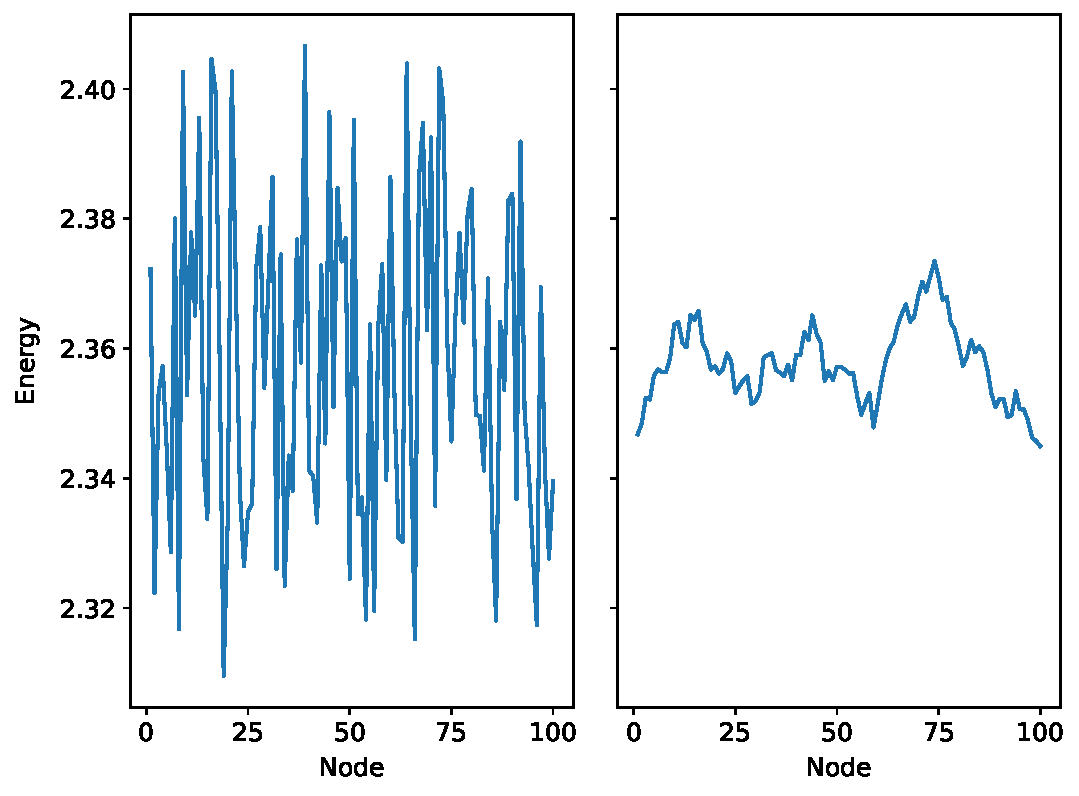
\includegraphics[width=0.7\columnwidth]{energyRoughSmooth.pdf} \\
    \hspace{0.5in} (a) \hspace{1.8in} (b)
    \caption{(a) The raw data trace of the system's energy alongside (b) the smoothed version.}
    \label{fig:energyRoughSmooth}
\end{figure}

To determine which of these predictions (at $t=0$) is better, we can examine the full-time evolution of the pendulum chain using these initial conditions, shown in Fig.~\ref{fig:colormap}. Here the horizontal axis is spatial (i.e., the 100 pendulums), the vertical axis is computational time, and the color depicts the angle in panel (a), and the energy in panel (b). We see that eventually the energy sharply localizes on pendulums 70-72, and so it is clear that smoothing the energy resulted in a much better prediction.

\begin{figure}
    \centering
    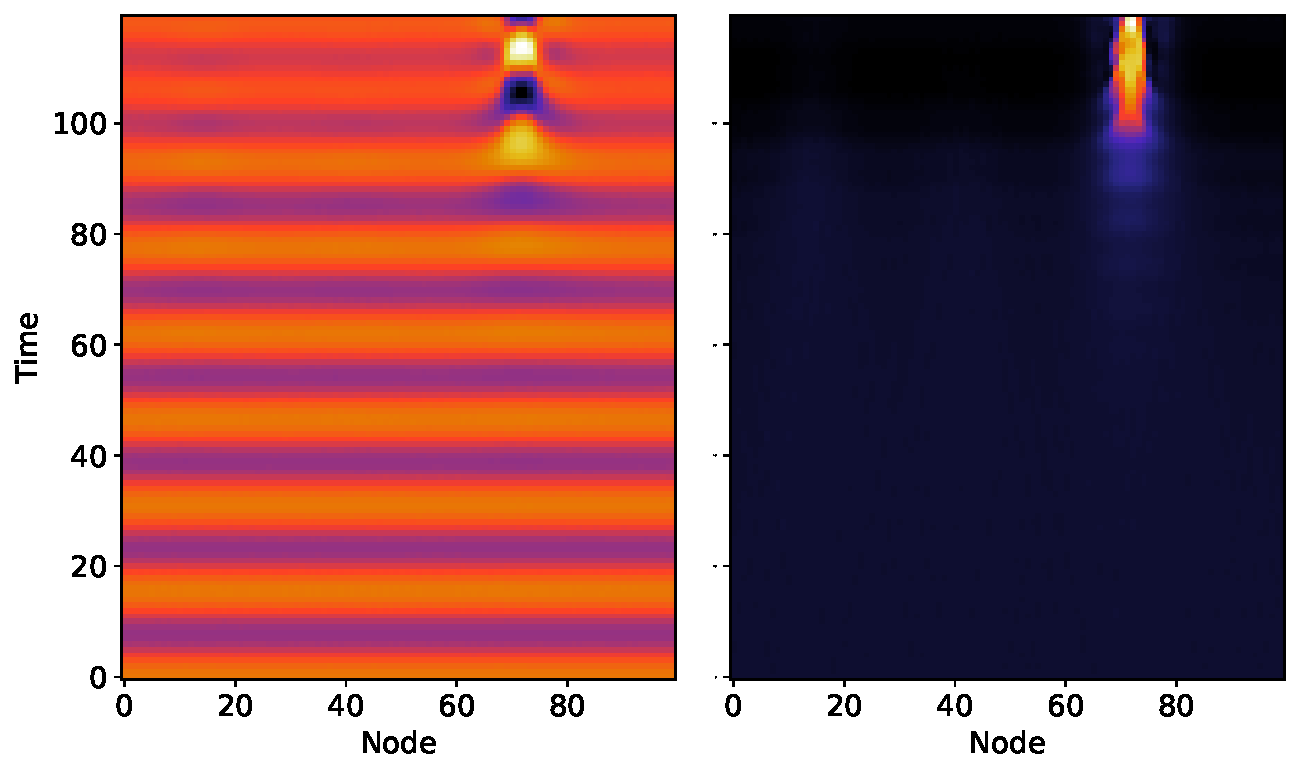
\includegraphics[width=0.75\columnwidth]{colormap.pdf}
    \\
     \hspace{0.3in} (a) \hspace{2.1in} (b)
    \caption{Color-map of (a) angle and (b) energy oscillation for the entire simulation}
    \label{fig:colormap}
\end{figure}

\subsection{Localization Time}

\begin{figure}
    \centering
    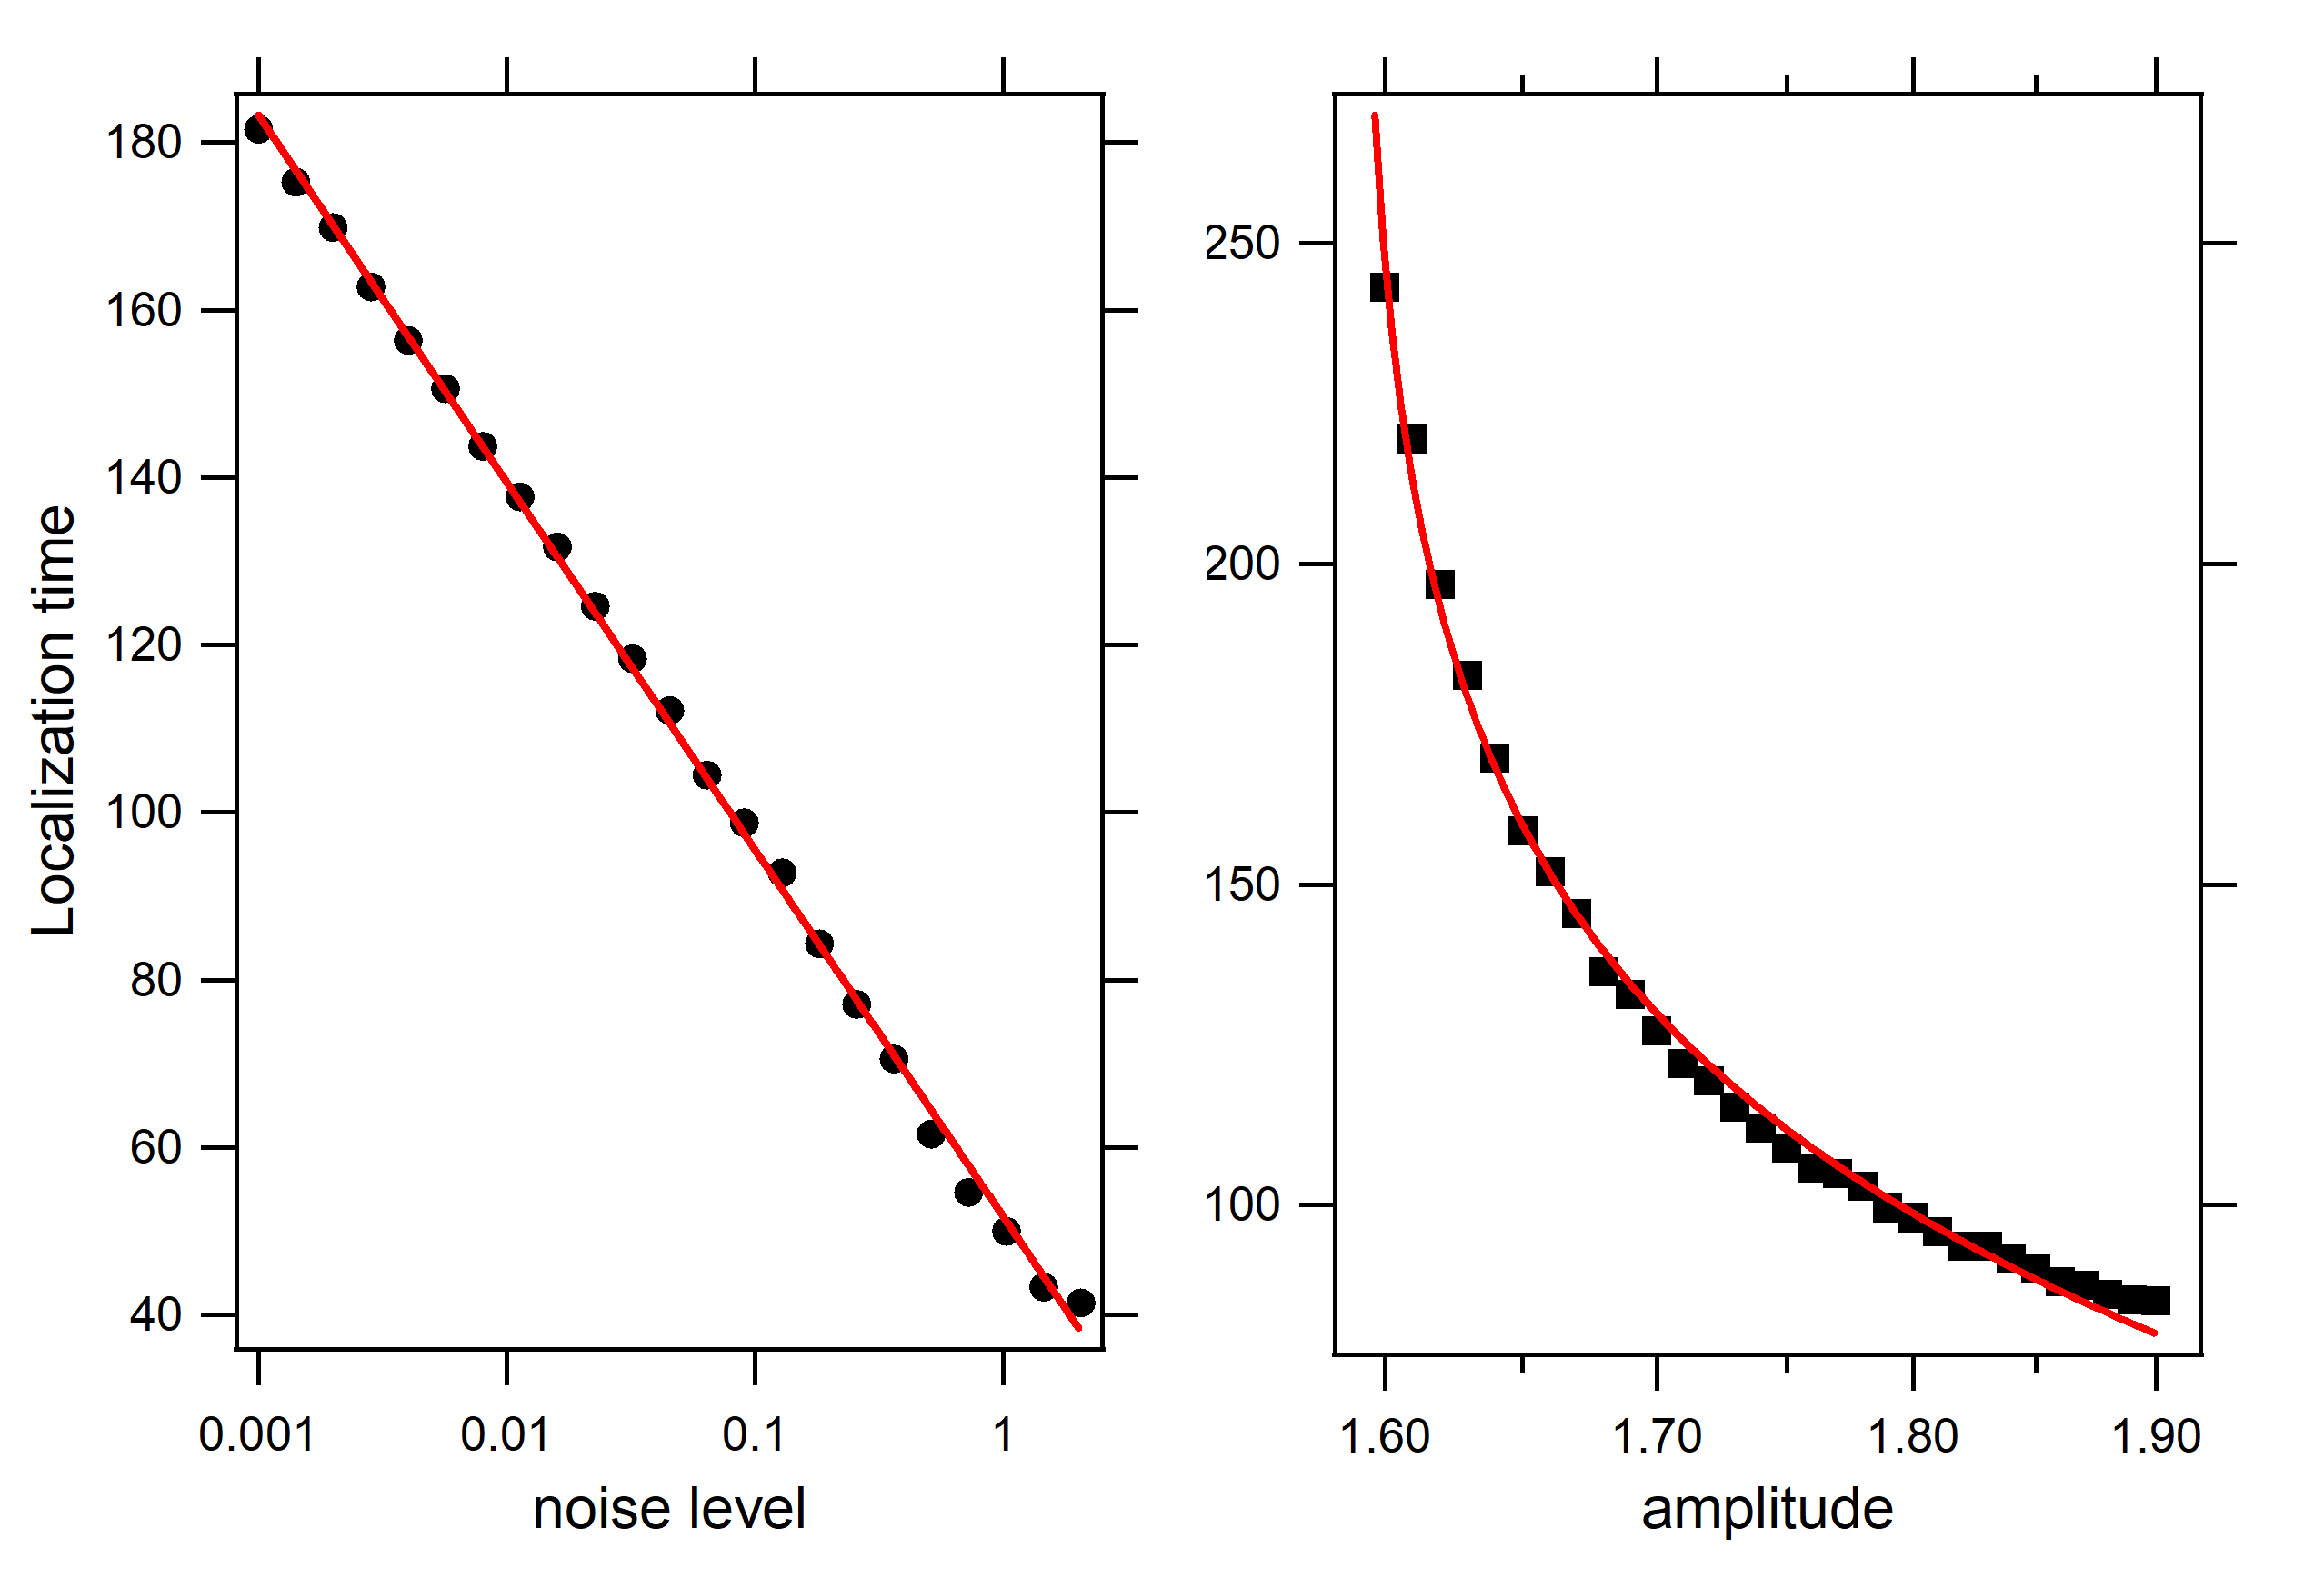
\includegraphics[width=0.7 \columnwidth]{loc_time.png} \\
     \hspace{0.3in} (a) \hspace{2.0in} (b) 
    \caption{Dependence of the average localization time on initial noise level and amplitude of the oscillation in the chain. (a) The dependence on noise level is seen as logarithmic. (b) The amplitude dependence features a vertical asymptote at around A=1.59 indicating the instability's amplitude threshold.}
    \label{fig:loc_time}
\end{figure}
By visual inspection of Fig.~\ref{fig:colormap}, we see that sharp energy localization happens fairly abruptly around a timestamp of $t \approx 100$. We now briefly address the question of what determines this timescale. There are two adjustable parameters in the way the system is initialized, namely the noise level and the initial angular displacement (or amplitude). 

To understand how changing these two parameters affects the localization time, we calculated the average localization time over 100 simulations for a series of different noise levels and amplitudes.

Let us first look at the role of noise.
Figure \ref{fig:loc_time}(a) depicts the time it takes the system to first concentrate 10 percent of its total energy on a single pendulum, as a function of noise level (plotted on a logarithmic axis). There is an exponential relationship between these two quantities - the larger the noise the quicker the localization happens. Since the pattern-formation process is noise-activated, this relationship is expected; nonetheless, the precise exponential relationship (given by the straight line in the logarithmic plot) uncovered numerically is remarkable.

In Fig.~\ref{fig:loc_time}(b), the relationship between localization time and initial pendulum amplitude is illustrated. As expected, here we get a vertical asymptote at around $A=1.59$ due to the amplitude threshold exhibited by this type of instability. (The solid line is a negative logarithmic function to guide the eye.)

\subsection{Prediction quality using only data smoothing}
\label{sec:smoothing}
We are now ready to explore the prediction quality of energy localization based on a hypothesis that the type-III pattern-formation process is guided by random clusters of higher energy. Here, our major question pertains to the optimal kernel size in the smoothing algorithm. Figure \ref{fig:smoothResults} summarizes our numerical findings. It plots the mean absolute difference between the predicted and actual location against the time of prediction (or ``timestamp'') for each of the 7 different kernel sizes. Note that the error bars are included in the graph but so small that they are not readily visible.
\begin{figure}
    \centering
    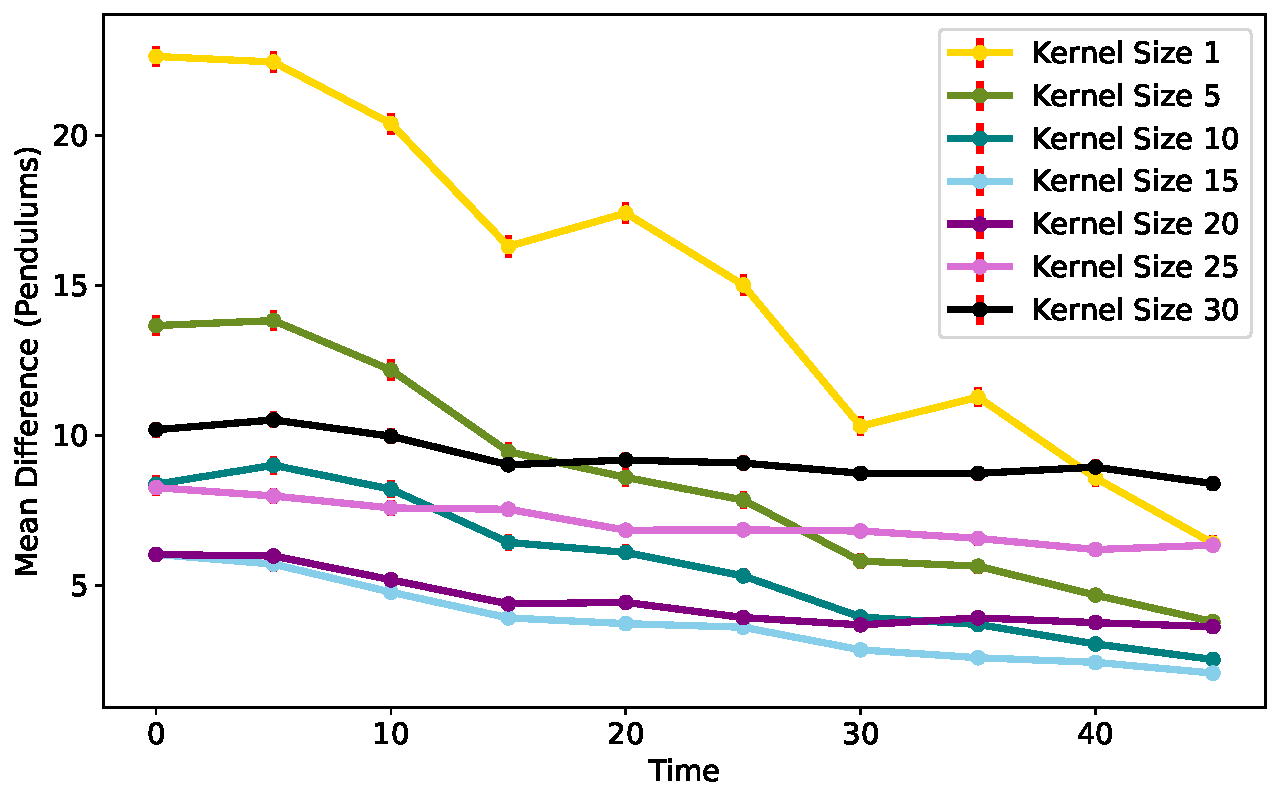
\includegraphics[width=0.6\columnwidth]{finalResults.pdf}
    \caption{Mean Difference vs Time for kernel sizes ranging from 1 to 30. Each series shows the absolute difference between a certain kernel size's prediction and the actual localization site, and how this difference changes as the time at which the prediction is made progresses.}
    \label{fig:smoothResults}
\end{figure}

A few trends can immediately be observed from this graph. The clearest trend is that as time progresses the accuracy of the predictions increases for most of the kernel sizes. This makes sense because the closer the prediction occurs to the real event, the more accurate one would expect it to be. Note that the localization event occurred around a timestamp of 100.

Secondly, the kernel size with the worst accuracy at almost every timestamp is 1. A kernel size of 1 is equivalent to the raw (non-smoothed) energy data, which clearly demonstrates that using a moving average substantially increases the accuracy of predictions. Kernel sizes of about 12-18 seem to be the most accurate over a broad range of times.

To delve deeper into the effect of different kernel sizes, we examined the relationship between kernel size and mean difference at a timestamp of 5. This is effectively the same as examining the columns of data points corresponding to 5 on the horizontal axis in Fig.~\ref{fig:smoothResults}. 
\begin{figure}
    \centering
    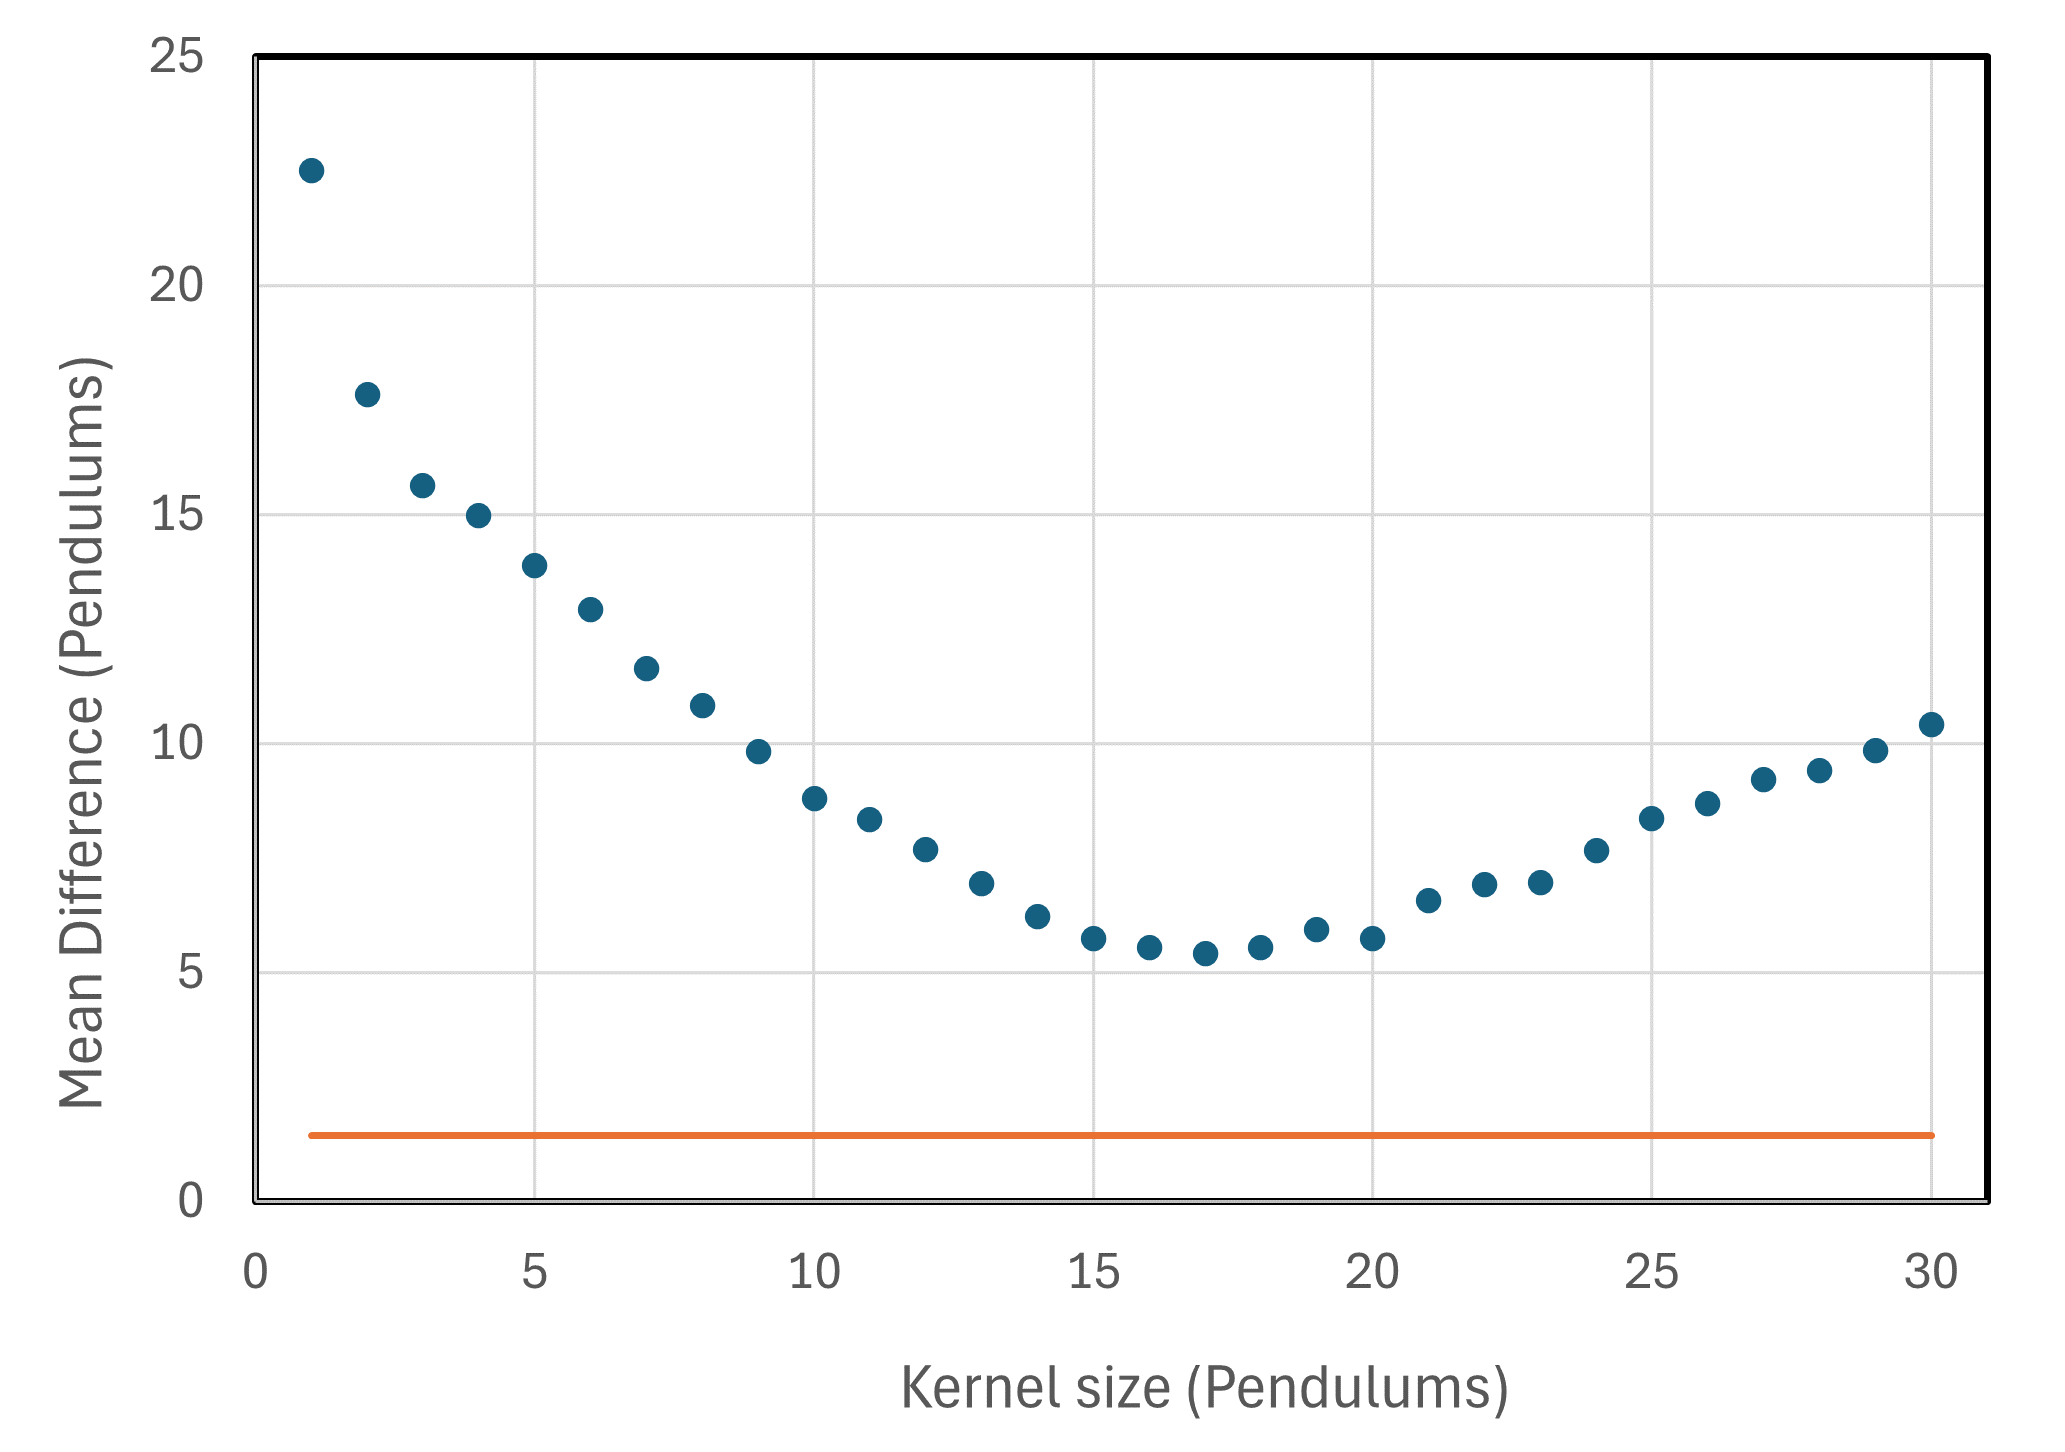
\includegraphics[width=0.6\columnwidth]{fig5n.png}
    \caption{Mean Difference vs Kernel Size at a timestamp of $t=5$. A lower mean difference entails a higher prediction quality and vice versa. The circles represent the mean difference for each kernel size (smoothing window size). We see that the best prediction occurs for a kernel size in the range of 15-20. The solid line below the circles represents the mean difference achieved by ML, as discussed later. The kernel size on the horizontal axis applies only to the box-car smoothing; the solid line does not depend on it.}
    \label{fig:5_45_timePlot}
\end{figure}

Figure \ref{fig:5_45_timePlot} plots the mean absolute difference as a function of kernel size (smoothing window size) at a prediction timestamp of $t=5$, with each data point representing the average of 2000 simulations. Notice the sharp improvement in prediction as the kernel size is increased from 1 to about 10. A minimum is then reached just after 15, past which the prediction gets worse again. Thus, smaller kernel sizes are inaccurate due to the insufficient smoothing of the spatial noise, and the larger kernel sizes are unable to reach pinpoint accuracy due to an over-smoothing of important spatial features in the energy landscape. The optimal range of kernel sizes (to maximize the prediction accuracy) is from 15 to 20, with the best kernel size occurring at 17. 

We conclude that the noise-sensitive process whereby the initial instability of type III gives rise to an energy hotspot is sensitive to energetic clusters comprising 10-15 pendulums. In other words, an initial region of elevated energy over that length scale will likely produce an energy hotspot in that same region later in time. Interestingly, a single pendulum of large energy is not nearly as determinative of the eventual localization region.

\subsection{Machine-Learning Results}

To evaluate the efficacy of our machine-learning approach, we assessed the CNN-LSTM model's performance on a test set of 20,000 simulations, focusing on its ability to predict both the occurrence of energy localization (localization accuracy) and the specific pendulum where it occurs (location accuracy). The model was trained on early-time data (first 10 timesteps, $0 \leq t \leq 4.5$), using initial angular displacements and per-pendulum energy profiles as features. As before, localization was defined as a pendulum's energy exceeding 10\% of the total system energy, with the first such instance determining the localization site and time.

For location accuracy, we adopted a tolerance of $\pm 1$ pendulum, reflecting the spatial extent of energy localization, which typically spans multiple pendulums. The model predicted the localization site within $\pm 1$ pendulum of the true location in $94.38\%$ of cases where localization occurred, with an average absolute error of 1.44 pendulums across 20,000 test simulations. Notably, 94.38\% of predictions had an error of $\leq 1$ pendulum, with rare outliers skewing the average error slightly higher - see Fig.~\ref{fig:dist}.

\begin{figure}
    \centering
    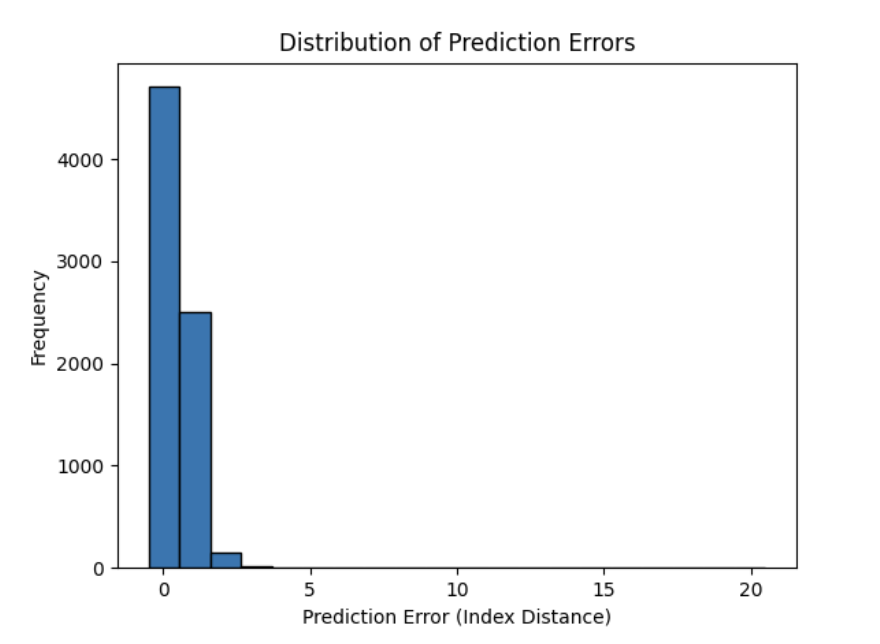
\includegraphics[width=0.6\linewidth]{Distribution-of-pred-errors.png}
    \caption{Distribution of Prediction Errors}
    \label{fig:dist}
\end{figure}

To contextualize these results, we compare them to the physics-inspired smoothing approach (Section~\ref{sec:smoothing}). At a timestamp of $t = 5$, the optimal smoothing kernel size of 17 yielded a mean absolute difference of approximately 5.4 pendulums (Fig.~\ref{fig:5_45_timePlot}). 

In contrast, our machine-learning model, using only $t \leq 4.5$ data, achieved a mean error of 1.44 pendulums, representing a 3.75-times improvement over the best smoothing results at early times. This improvement over the physics-inspired method is illustrated graphically in Fig.~\ref{fig:5_45_timePlot} by the solid (orange) line, which lies significantly below markers from the smoothing-procedure prediction. 

These results underscore the machine-learning model's ability to capture complex spatial and temporal patterns in the sine-Gordon system’s early chaotic dynamics (see also Ref.\cite{Chaos_Ott_2017,PhysRevLett_Ott_2018}), beyond the energy clusters identified by smoothing. The CNN layers likely extract localized spatial features, while the bidirectional LSTM captures temporal evolution, enabling robust predictions despite the system’s chaotic sensitivity to initial conditions. The high accuracy at early times ($t \leq 4.5$, well before the typical localization time of $t \approx 100$) suggests that the model identifies subtle precursors to type-III instabilities, potentially including higher-order correlations or nonlinear interactions not captured by smoothing alone.

The dramatic improvement over smoothing and traditional methods highlights the potential of data-driven approaches for predicting chaotic dynamics. The superior performance of machine learning shows that our neural network has discovered some hidden temporal and spatial dependencies that traditional physics methods did not uncover. By leveraging only early-time data, our model offers a practical tool for forecasting energy localization, with applications in mitigating structural instabilities in engineering systems. Future analyses will aim to interpret the learned features, potentially revealing new physical insights into type-III instabilities and their precursors.

\subsection{The Role of Impurities}

An unavoidable issue in any macroscopic physical lattice is spatial inhomogeneity. One form of inhomogeneity is the appearance of an impurity somewhere in the lattice, where one lattice element is slightly different from the others. We now examine the role of such an impurity in the pattern formation process. In particular, we study how changing the impurity strength affects where energy localizes and how long it takes to form in time. In our simulations, we set pendulum number 50 as the only pendulum with an impurity in order to showcase the effect of even one impurity in the chain. The impurity was introduced in the on-site term of the sine-Gordon model. Instead of the second term of Eq.~(\ref{sG}) starting with $\omega_0^2$, for $n=50$ it starts with $(1-\epsilon)\omega_0^2$, where $0<\epsilon \ll 1$. In other words, the pendulum at the impurity is slightly lengthened relative to the others. Impurities of the opposite sign repel energy in this model. 


\begin{figure}
    \centering
    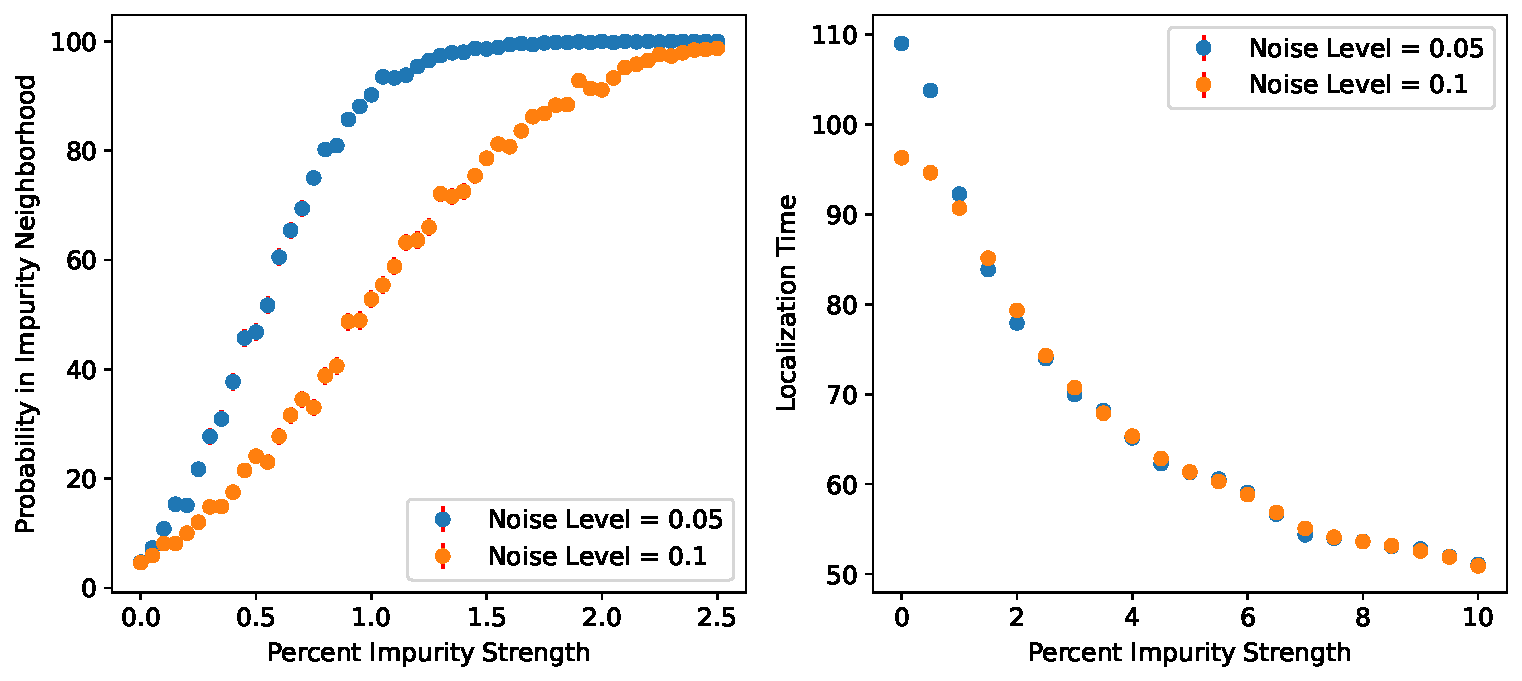
\includegraphics[width=1\columnwidth]{impurityPlot.pdf} \\
     \hspace{0.15in} (a) \hspace{3.2in} (b)
    \caption{(a) As the impurity strength is increased, the probability of energy localizing near the impurity site also increases and (b) the localization time decreases.}
    \label{fig:impurityPlot}
\end{figure}

When determining how impurities affect the location of energy we first notice that impurities of this kind (for $\epsilon>0$) significantly increase the probability that energy localizes around pendulum 50. In Fig.~\ref{fig:impurityPlot}(a), we graph the impurity strength against the probability that energy would localize in proximity to pendulum 50. For this data, the acceptable proximity was from pendulum 48 to pendulum 52, a range of 5. Figure \ref{fig:impurityPlot}(a) clearly shows a positive correlation between the percent impurity strength and energy localization in the impurity neighborhood. The two datasets (blue and orange) are for different values of the spatial noise in the initialization. Blue (orange) dots represent an initial noise level (relative to the oscillation amplitude) of 1.4 percent (2.8 percent).

For the lower spatial noise (blue markers), we see that from 0 percent to around 1 percent the relation is relatively linear, and from 1 percent onward, the probability of localization at the impurity site slowly approaches 100 percent. 
For larger spatial noise in the initialization, it takes a larger impurity strength to achieve the same probability. This makes intuitive sense, given that the spatial noise and the spatial impurity are competing effects in the pattern-formation process that leads to energy localization.

The impurity strength also has a significant impact on localization time. We can see that in Fig. \ref{fig:impurityPlot}(b), as the impurity strength increases the localization time decreases. However, the rate at which the localization time decreases also lessens with greater impurity strength, leading the localization time to asymptotically approach a value of around 50. Here we see that the noise level plays a less prominent role.

We thus find that oscillators with an impurity strength as low as 1 percent of an ideal oscillator, or $\epsilon=0.01$, can significantly alter the result of a simulation by skewing the location and time of energy localization. 

\section{Conclusions}
In this study, we investigated the noise-induced, type III instability that leads to a sharp localization of energy in a sine-Gordon model. Characteristic of a chaotic process, this energy-localization dynamics is highly sensitive to slight variations in initial conditions. Because of this, an important question emerged: can the eventual outcome of energy localization be predicted at early times, and what should be known/computed to improve such an early prediction? We started with the physics-informed hypothesis of energy-clusters, and found that smoothing the relevant variables such as the angles or energies (using a numerical box-car integrator) significantly improved the accuracy of the prediction. An optimal kernel size in that smoothing was around 15, suggesting that the instability process is most sensitive to spatial energy clusters of that size. 

We then turned to machine learning to ascertain whether further improvements in prediction accuracy were possible based on only early-time data. We found that training a CNN-LSTM network on energy data at early times ($0\le t \le 4.5$), together with knowledge of the initial conditions for angles (at $t=0$) yielded a dramatic improvement in prediction quality, relative even to the best-kernel smoothing procedure. This strongly suggests that there are additional features, beyond above-average energy clusters, that influence the instability dynamics. A future study will aim at teasing out relevant features uncovered via machine learning.

Finally, we found that even slight impurities in the chain significantly affect energy localization, in time and space. Spatial impurity and spatial noise are thus two competing forces in the pattern-forming process that lead to energy localization.

\section*{Acknowledgements}
We would like to acknowledge helpful discussions with Hana Zwick, Dr. Robert Malkin, and Prof. Lulu Wang. We also thank Anya English for help with an early version of the code.

\section*{Appendix: Model Architecture Details}
The machine learning model integrates convolutional and recurrent neural network components to predict energy localization in the sine-Gordon system. Here, we elucidate the function of each layer, the role of the \texttt{TimeDistributed} wrapper, the bidirectional nature of the LSTM, and the choice of activation functions.

The input layer accepts a 4D tensor of shape $(N_{\text{sim}}, 10, 100, 2)$, where $N_{\text{sim}}$ is the number of simulations, 10 is the number of timesteps, 100 is the number of pendulums, and 2 represents the energy $E_i(t)$ and initial angular displacement $\theta_i(0)$ (repeated across timesteps). This tensor encapsulates the spatiotemporal evolution of the system, with energy profiles capturing dynamic localization patterns and initial angles providing static context.

Four time-distributed 1D convolutional layers (\texttt{Conv1D}), with 32, 64, 128, and 256 filters, respectively, process the input. Each \texttt{Conv1D} layer applies a sliding window (kernel size 3) to extract spatial features, such as local energy peaks or angular correlations, across the 100 pendulums at each timestep. The \texttt{TimeDistributed} wrapper ensures that the convolutional operation is applied independently to each of the 10 timesteps, preserving temporal structure and producing a sequence of feature maps (e.g., shape $(N_{\text{sim}}, 10, 100, 32)$ for the first layer). The ``same'' padding maintains the spatial dimension (100 pendulums), enabling consistent feature extraction across layers. The rectified linear unit (ReLU) activation function, $f(x) = \max(0, x)$, is applied element-wise to introduce nonlinearity, enhancing the model's ability to learn complex patterns while mitigating vanishing gradient issues during training \cite{Goodfellow-et-al-2016}.

A time-distributed \texttt{Flatten} layer follows, reshaping each timestep’s feature map (e.g., $(100, 256)$ from the final \texttt{Conv1D}) into a 1D vector (e.g., 25,600 elements), yielding a tensor of shape $(N_{\text{sim}}, 10, 25600)$. This preserves the temporal sequence for recurrent processing while consolidating spatial features.

The bidirectional long short-term memory (LSTM) layer, with 128 units, processes the sequence of flattened feature vectors to capture temporal dependencies in the energy and angle dynamics. An LSTM unit maintains a cell state and gates (input, forget, output) to selectively remember or forget information across timesteps, making it suitable for modeling the sequential evolution of localization \cite{Hochreiter1997}. Bidirectionality involves two LSTM layers: one processing the sequence forward (timesteps 0 to 9) and another backward (9 to 0), concatenating their outputs. This enables the model to learn both past and future contexts, crucial for identifying localization events that may depend on early and late timestep patterns. Dropout $(20\%)$ and recurrent dropout $(20\%)$ are applied to prevent overfitting by randomly masking inputs and recurrent connections during training.

A dense layer with 64 units and ReLU activation aggregates the LSTM output, reducing dimensionality and learning higher-level features for classification. Two output layers follow:
\begin{itemize}
\item The localization output, a dense layer with 1 unit and sigmoid activation, $f(x) = 1 / (1 + e^{-x})$, produces a probability (0 to 1) for binary classification (localization vs. no localization). Sigmoid is chosen for its bounded output, suitable for binary tasks.
\item The location output, a dense layer with 100 units and softmax activation, $f(x)_i = e^{x_i} / \sum_{j=1}^{100} e^{x_j}$, yields probabilities over the 100 pendulums, representing the likelihood of localization at each site. Softmax ensures normalized probabilities, ideal for multi-class classification.
\end{itemize}

The ReLU activation in convolutional and dense layers facilitates efficient gradient propagation and sparsity, while sigmoid and softmax activations align with the binary and multi-class nature of the outputs, respectively. The model’s architecture, combining spatial feature extraction (CNN), temporal modeling (bidirectional LSTM), and robust classification (dense layers), effectively captures the complex dynamics of energy localization in the sine-Gordon system.

Model performance was assessed on the test set using the total loss (weighted sum of localization and location losses), localization loss, location loss, localization accuracy, and location accuracy.  


\section*{Changes from the published version}
This version differs from the article published in J.\ Appl.\ Nonlinear Dyn.\ \textbf{15}(2), 277--290 (2026) only in the following corrections:
\begin{itemize}
\item Sec.~2.1: the global coupling is $\tilde{h}=0.5$ (printed as 0.05), the value used in all simulations and stated in Sec.~2.3.
\item Eq.~(6): the summation index is written explicitly.
\item Sec.~1: the network is a CNN combined with a bidirectional LSTM (printed as ``LSTM transformer'').
\item Sec.~3.3: Fig.~4 shows 7 kernel sizes (printed as 6); the caption of Fig.~5 is reworded for clarity.
\item Sec.~3.4: a cross-reference to Sec.~3.3 is corrected (printed as ``Section III.C'').
\item Sec.~4: the network's input window is $0\le t\le 4.5$ and the network is a CNN-LSTM (printed as $0\le t\le 5$ and ``CNN'').
\item Spelling, punctuation, code-name formatting, list formatting and reference capitalization.
\end{itemize}

% References: refs.bib with the journal's cj.bst. arXiv does not run BibTeX, so main.bbl is shipped.
\bibliographystyle{cj}
\bibliography{refs}

\end{document}